% !TEX program = xelatex
% Mixed raster/vector. Source: locked Jan20 2022 author PDF, pp11-14/S3/S5/S6.
% Generated viewports supply illustrations only; equations/arrows are independently checked.
\documentclass[tikz,border=2mm]{standalone}
\usepackage{fontspec,xeCJK,amsmath,amssymb,graphicx}
\setsansfont{Arial}
\setCJKmainfont[Path=/System/Library/Fonts/,BoldFont={STHeiti Medium.ttc}]{STHeiti Light.ttc}
\setCJKsansfont[Path=/System/Library/Fonts/,BoldFont={STHeiti Medium.ttc}]{STHeiti Light.ttc}
\renewcommand{\familydefault}{\sfdefault}
\usetikzlibrary{arrows.meta,calc}
\definecolor{ink}{HTML}{173646}
\definecolor{teal}{HTML}{217E80}
\definecolor{amber}{HTML}{B5712F}
\definecolor{purple}{HTML}{735098}
\definecolor{pale}{HTML}{F6F8F7}
\definecolor{warm}{HTML}{FFF6E9}
\definecolor{violet}{HTML}{F3EFF9}
\tikzset{t/.style={text=ink,font=\fontsize{16.5}{20}\selectfont,align=center,inner sep=0},
 hd/.style={t,font=\bfseries\fontsize{21}{25}\selectfont},
 sm/.style={t,font=\fontsize{15}{18}\selectfont},
 a/.style={-{Stealth[length=3mm,width=2mm]},line width=1.4pt,draw=teal,rounded corners=2pt},
 sup/.style={a,draw=amber,dashed},
 box/.style={rounded corners=4pt,line width=.8pt}}
\newcommand{\txt}[4]{\node[t,text width=#3cm]at(#1,#2){#4};}
\newcommand{\head}[4]{\node[hd,text width=#3cm]at(#1,#2){#4};}
\newcommand{\smalltxt}[4]{\node[sm,text width=#3cm]at(#1,#2){#4};}
\newcommand{\maths}[4]{\node[text=ink,font=\fontsize{#3}{#3}\selectfont,inner sep=0]at(#1,#2){\(\displaystyle #4\)};}
\newcommand{\panel}[7]{\draw[box,draw=#6!45,fill=#7](#1,#2)rectangle++(#3,#4);\pgfmathsetmacro{\pw}{#3-.3}\head{#1+#3/2}{#2+.47}{\pw}{#5}}
% Source PNG has 1536x1024 pixels and 72dpi natural size. Unmodified viewports.
\newcommand{\art}[7]{\begingroup\pgfmathsetmacro{\bt}{1024-#2-#4}\pgfmathsetmacro{\rt}{1536-#1-#3}
\node[anchor=north west,inner sep=0]at(#5,#6){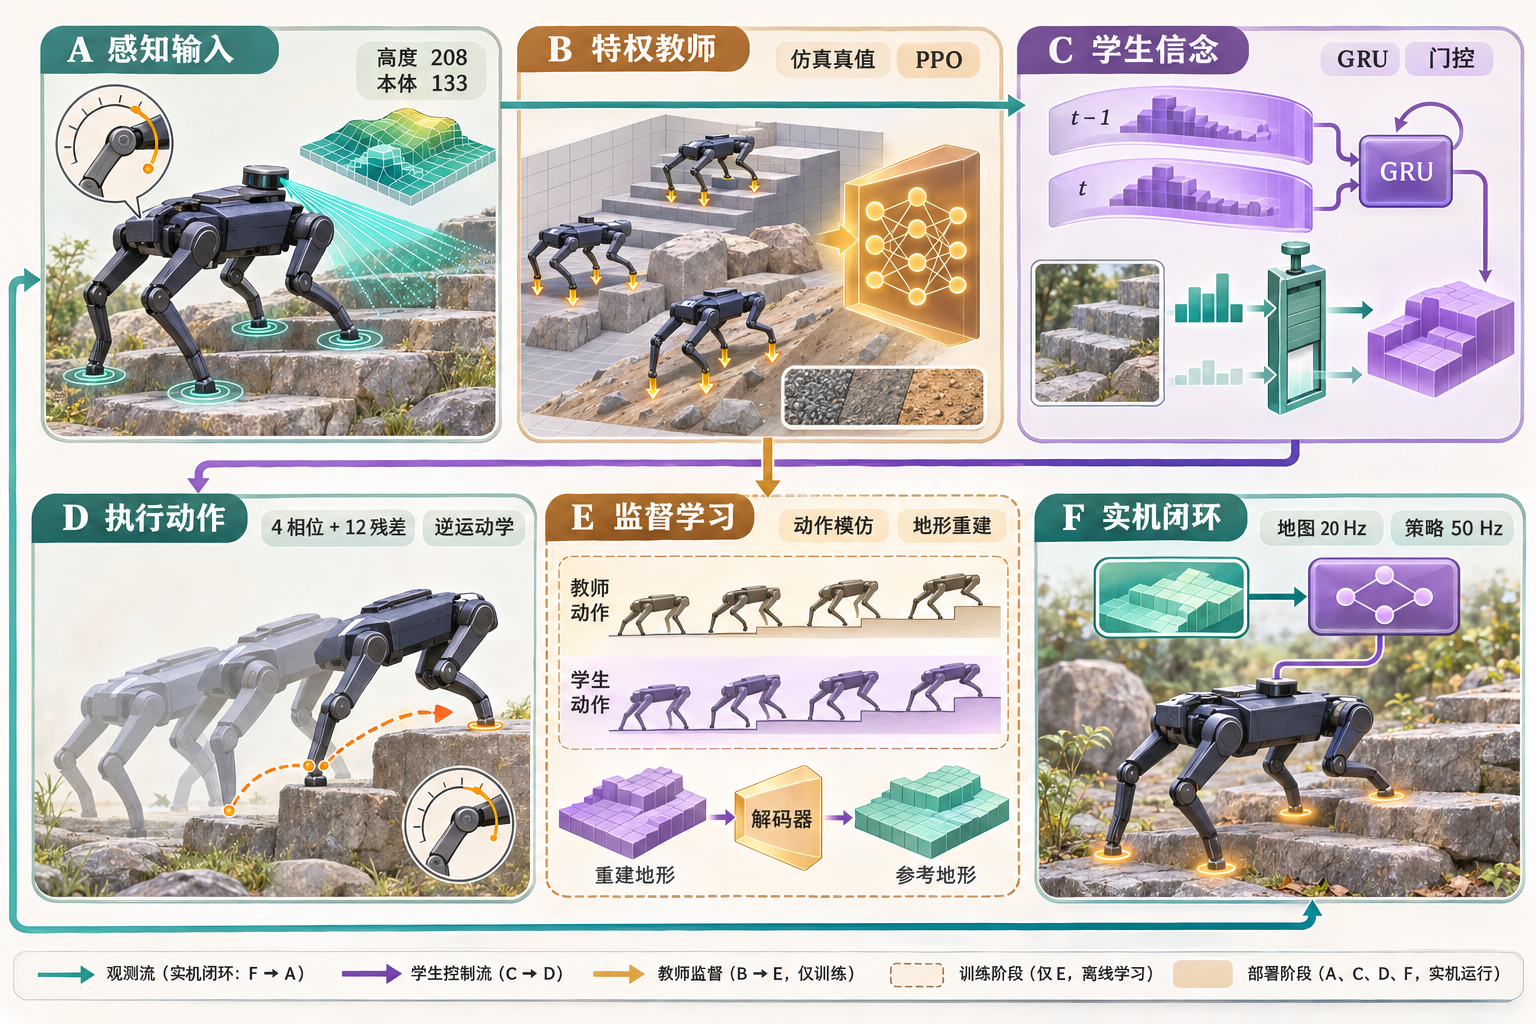
\includegraphics[trim=#1bp \bt bp \rt bp #2bp,clip,width=#7cm]{perceptive-loco-imagegen-draft.png}};\endgroup}
\begin{document}
\begin{tikzpicture}[x=1cm,y=-1cm]
\path[use as bounding box](0,0)rectangle(12.5,20.8);\fill[white](0,0)rectangle(12.5,20.8);
\head{6.25}{.5}{12}{B / E\quad 教师怎样带学生？}
\art{523}{113}{464}{320}{.65}{1.15}{5.4}
\art{559}{556}{449}{192}{6.45}{1.5}{5.4}
\txt{6.25}{5.37}{11.4}{先用 PPO 训练教师，再固定教师产生标签}
\draw[box,draw=amber!50,fill=warm](.4,6.0)rectangle(12.1,9.45);
\txt{6.25}{6.6}{11}{学生 rollout，访问它实际走到的状态}
\txt{6.25}{7.35}{11}{同一状态、同一速度指令：比较两方动作}
\maths{6.25}{8.35}{21}{\mathcal L_{bc}=\|a_t^S-a_t^T\|_2^2}
\draw[sup](12.1,8.35)--(12.35,8.35)--(12.35,16.05)--(12.1,16.05);
\draw[box,draw=amber!50,fill=warm](.4,10.0)rectangle(12.1,14.7);
\txt{6.25}{10.62}{11}{循环隐藏状态 + 原始带噪高度 → 解码器}
\txt{6.25}{11.4}{11}{解码器有自己的门控支路}
\maths{6.25}{12.3}{18}{\mathcal L_{re}=\|[\widehat o_t^e,\widehat s_t^p]-[o_t^e,s_t^p]\|_2^2}
\txt{6.25}{13.3}{11}{目标：干净高度 208 + 特权量 50}
\smalltxt{6.25}{14.05}{11}{重建的是环境量，不是 120 维潜变量}
\draw[sup](6.25,14.7)--(6.25,15.25);
\draw[box,draw=amber!50,fill=warm](.4,15.25)rectangle(12.1,17.65);\maths{6.25}{16.05}{23}{\mathcal L=\mathcal L_{bc}+0.5\mathcal L_{re}}
\txt{6.25}{17.15}{11}{联合更新学生，保留有用的环境信息}
\draw[box,draw=teal!40,fill=pale](.4,18.0)rectangle(12.1,20.4);
\txt{6.25}{18.7}{11}{实机运行：只使用学生策略}
\txt{6.25}{19.65}{11}{教师与解码器退出。\\参数固定，隐藏状态更新。}
\end{tikzpicture}
\end{document}
